\documentclass[11pt, norsk]{article}
%\usepackage[latin1]{inputenc}
\usepackage[T1]{fontenc}
\usepackage[utf8]{inputenc}
\usepackage[norsk]{babel}   % S P R A A K

\usepackage{standalone}
\usepackage{graphicx}    % postscript graphics
\usepackage{amssymb, amsmath, amsthm, amssymb} % symboler, osv
\usepackage{mathrsfs}
\usepackage{url}
\usepackage{thmtools}
\usepackage{enumerate}  % lister $  
\usepackage{float}
\usepackage{tikz}
\usetikzlibrary{decorations.pathmorphing}
\usetikzlibrary{calc}
\usetikzlibrary{intersections}
\usepackage{tikz-3dplot}
\usepackage{subcaption}
\usepackage[all]{xy}   % for comm.diagram
\usepackage{wrapfig} % for float right
\usepackage{hyperref}
\usepackage{mystyle} % stilfilen      


\begin{document}
\title{Oppgaver MAT2500}
\author{Fredrik Meyer}
\maketitle 

\begin{oppg}
La $P=(1:0:0)$, $Q=(1:1:0)$, $R=(1:0:1)$ og $S=(1:1:1)$ være punkter i $\PP^2_\R$. Regn ut snittet av $\ol{PQ}$ og $\ol{RS}$.
\end{oppg}
\begin{losn}
Vi finner først ligningen for linjen $\ol{PQ}$. Den mekaniske måten er å skrive ut determinanten
$$
\begin{vmatrix}
 x_0 & x_1 & x_2 \\
 1 & 0 & 0 \\
1 & 1 & 0
\end{vmatrix} = 0
$$
Vi får $x_2=0$, som vi kunne gjettet oss til ved å se på punktene (...).

Tilsvarende finner vi at $\ol{RS}$ er gitt ved $x_0-x_2=0$ (dette er riktig fordi ligningen $x_0-x_2=0$ definerer en projektiv linje, og $R,S$ begge ligger på denne linjen).

Dermed er snittet deres gitt av ligningssystemet $x_2=0, x_0-x_2=0$. Altså $x_0=x_2=0$. Med andre er snittet lik punktet $(0:1:0)$. 
\end{losn}

\begin{oppg}
Lag et projektiv plan med 13 punkter og 13 linjer.
\end{oppg}

\begin{losn} 
Dette er vanskeligere enn det høres ut som. Mange har kanskje sett Fano-planet med syv elementer. Se Figur 1.
\begin{figure}
 \centering
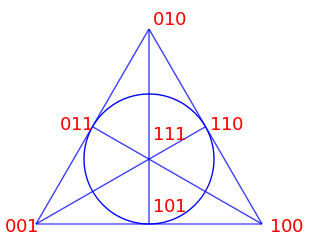
\includegraphics[width=90mm]{fanoplane}
  \caption{Fano-planet.}
\end{figure}  
Legg merke til at koordinatene. Legger du sammen to punkter på sammme linje får du det tredje punktet, så dette er en spesielt pen framstilling.

Det finnes også et projektiv plan med $13$ elementer. Én mulighet er å tegne det på samme måte som Fano-planet, altså som en trekant med homogene koordinater og standardkoordinatene $(1:0:0),(0:1:0)$ og $(0:0:1)$ på hjørnene. Dessverre blir ikke dette bildet på langt nær så pent som Fano-planet. Se Figur 2 og 3 for to muligheter.
\begin{figure}
  \centering
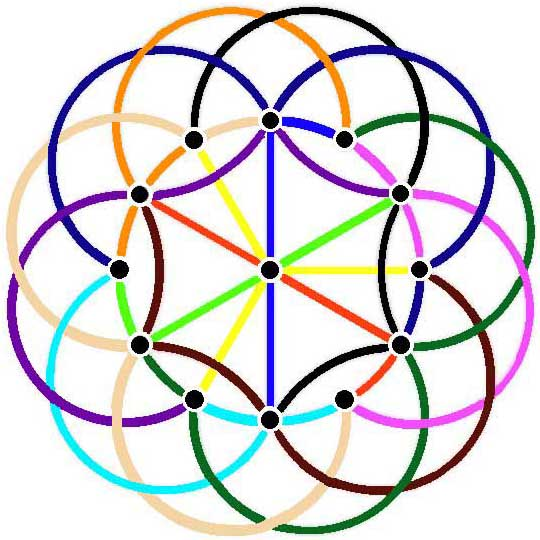
\includegraphics[width=90mm]{projplane13.jpg}
  \caption{En veldig symmetrisk framstilling av $\PP^2_{\mathbb F_3}$.}
\end{figure}
\begin{figure}
\centering
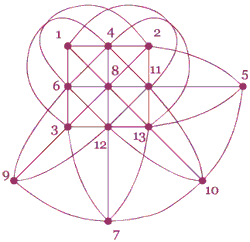
\includegraphics[width=90mm]{proj132}
  \caption{En annen, kanskje mer oversiktlig framstilling.}
\end{figure}
Vi ser at Figur 2 er mer symmetrisk, men Figur 3 er mer oversiktlig. 

I Figur 4 er en versjon jeg laget, modellert etter den vanlige framstillingen av Fano-planet. Linjene blir ganske uoversiktlige, men om man studerer dette, ser man en del symmetri. 
\begin{figure}
%\documentclass[11pt, english]{article}
\documentclass{standalone}
%\usepackage[latin1]{inputenc}
\usepackage[T1]{fontenc}
\usepackage[utf8]{inputenc}
%\usepackage[english]{babel}   % S P R A A K


% \usepackage{graphicx}    % postscript graphics
\usepackage{amssymb, amsmath, amsthm, amssymb} % symboler, osv
\usepackage{mathrsfs}
%\usepackage{url}
%\usepackage{thmtools}
%\usepackage{enumerate}  % lister $  
%\usepackage{float}
\usepackage{tikz}
\usetikzlibrary{decorations.pathmorphing}
\usetikzlibrary{calc}
\usetikzlibrary{intersections}
%\usepackage{tikz-3dplot}
%\usepackage{subcaption}
%\usepackage[all]{xy}   % for comm.diagram
%\usepackage{wrapfig} % for float right
%\usepackage{hyperref}
%\usepackage{mystyle} % stilfilen      


\begin{document}

%\begin{figure}
%\begin{center}
  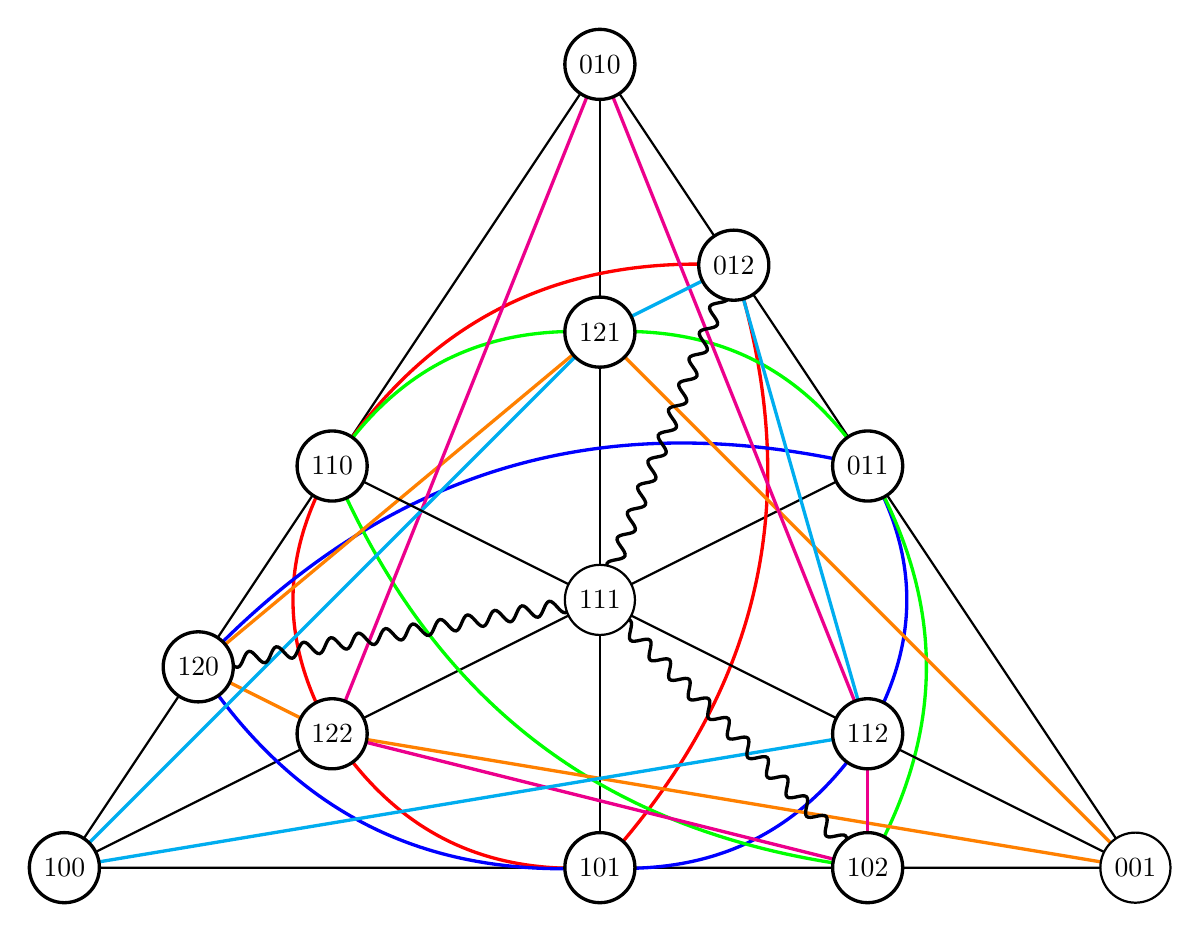
\begin{tikzpicture}[scale=1.7,every node/.style={circle, draw=black, fill=white}, every path/.style={very thick}]
\coordinate (A) at (-4,0);
\coordinate (B) at (4,0);
\coordinate (C) at (0,6);	
\coordinate (D) at (0,0);
\coordinate (E) at (2,0);
\coordinate (F) at (-2,3);
\coordinate (G) at (2,3); % 011
\coordinate (H) at (1,4.5);
\coordinate (I) at (-3,1.5);
\coordinate (J) at (0,2);
\coordinate (K) at (-2,1);
\coordinate (L) at (0,4);
\coordinate (M) at (2,1);

\draw[thick] (A) -- (B)  -- (C) -- cycle;  %1
\draw[thick] (A) -- (K) -- (J) -- (G);   % 2
\draw[thick] (C) -- (L) -- (J) -- (D); % 3
%
\draw[color=red] (D) to[bend left] (K); %1
\draw[color=red] (K) to[bend left] (F);
\draw[color=red] (F) to[bend left] (H);
\draw[color=red] (H) to[bend left] (D);
%
\draw[color=blue] (D) to[bend left] (I); %2
\draw[color=blue] (I) to[bend left] (G);
\draw[color=blue] (G) to[bend left] (M);
\draw[color=blue] (M) to[bend left] (D);
%
\draw[color=green] (E) to[bend left] (F); %3
\draw[color=green] (F) to[bend left] (L);
\draw[color=green] (L) to[bend left] (G);
\draw[color=green] (G) to[bend left] (E);
%
\draw[color=orange] (I) to (L); %5
\draw[color=orange] (L) to (B);
\draw[color=orange] (B) to (K);
\draw[color=orange] (K) to (I);
%
\draw[color=magenta] (C) to (M); %6
\draw[color=magenta] (M) to (E);
\draw[color=magenta] (E) to (K);
\draw[color=magenta] (K) to (C);
%
\draw[color=cyan] (A) to (L); %7
\draw[color=cyan] (L) to (H);
\draw[color=cyan] (H) to (M);
\draw[color=cyan] (M) to (A);
%

\draw[decorate, decoration={snake}] (J) -- (I);
\draw[decorate, decoration={snake}] (J) -- (H);
\draw[decorate, decoration={snake}] (J) -- (E);

\draw[thick] (J) node {111} -- (B) node {001} -- (F); % 11
\draw (A) node {100};
\draw (C) node {010};
\draw (D) node {101};
\draw (E) node {102};
\draw (F) node {110};
\draw (G) node {011};
\draw (H) node {012};
\draw (I) node {120};
\draw (K) node {122};
\draw (L) node {121};
\draw (M) node {112};
\end{tikzpicture}
%\caption{The projective plane $\PP_{\F_3}^2$.}
%\end{center}
%\end{figure}



\end{document}

  \caption{Det projektive planet $\PP_{\F_3}^2$.}
\end{figure}
\end{losn}

\begin{oppg}
 Det projektive plan med $13$ punkter og $13$ linjer er $\PP_{\F_2}^2$, der $\F_2$ er kroppen med tre elementer (altså addisjon og multiplikasjon modulo tre). Vi har homogene koordinater $(x_0:x_1:x_2)$ der $x_i \in \F_2$, akkurat som i $\PP_\R^2$.

Vis at man kan indeksere punktene $P_0,\ldots, P_{12}$ og linjene $\ell_0,\ldots,\ell_{12}$ slik at $P_i \in \ell_j$ hvis og bare hvis $i + j \equiv 0,1,3,9 \pmod{13}$. Lag en $13 \times 13$-matrise $A$ med $A_{ij}=1$ hvis $P_i \in \ell_j$ og $0$ ellers.
\end{oppg}
\begin{losn}
  Vi hopper foreløpig over denne.
\end{losn}

\begin{oppg}
  Med notasjonen fra forrige oppgave, vis at trekantene $P_1P_2P_7$ og $P_3P_8P_4$ er i perspektiv fra $P_0$, det vil si at linjene $\ol{P_1P_3}$, $\ol{P_2P_8}$ og $\ol{P_7 P_4}$ alle går gjennom $P_0$. 

Verifiser Desargues teorem i dette tilfellet. Det vil si, finn $\ol{P_1P_2} \cap \ol{P_3 P_8}$, $\ol{P_2 P_7} \cap \ol{P_4P_8}$ og $\ol{P_3P_4} \cap \ol{P_1P_7}$, og vis at de ligger på en linje.
\end{oppg}
\begin{losn}
Vi gjør en variant av oppgaven. Velg $P_1,P_2,P_7$ til å være de ytre hjørnene i Figur 4. Det vil si, $P_1=(1:0:0)$, $P_2=(0:0:1)$ og $P_7=(0:1:0)$. 

Tilsvarende la $P_3,P_8,P_4$ være den ``indre'' trekanten, altså punktene $(1:2:2),(1:1:2)$ og $(1:2:1)$. 

Da ser vi fra figuren at om vi lar $P_0=(1:1:1)$, så er trekantene i perspektiv fra $P_0$. En annen måte er å finne ligningene til de forskjellige linjene. For eksempel er linjen $\ol{P_1P_3}$ gitt ved $x_1=x_2$.

Nå kan vi se fra bildet at snittene $\ol{P_1P_2} \cap \ol{P_3P_8}$, $\ol{P_2 P_7} \cap \ol{P_4P_8}$ og $\ol{P_3P_4} \cap \ol{P_1P_7}$ er henholdsvis $(1:0:2), (0:1:2)$ og $(1:2:0)$. Men disse ligger alle på den buete linjen, altså linjen $x_0+x_1+x_2=0$.

Vi konkluderer med at Desargues teorem holder (ihvertfall for disse to trekantene).
\end{losn}

\begin{oppg}
 En perspektivitet med senter $C \in \PP_\R^2$ er en avbildning ${\alpha:\ell \to \ell'}$ mellom to linjer i $\PP_\R^2$ som sender $P \in \ell$ til $\ol{PC} \cap \ell'$. Vis at $\alpha$ er bijektiv, at det finnes nøyaktig ett fikspunkt, og at $\alpha^{-1}$ også er en perspektivitet.
\end{oppg}
\begin{losn}
Se Figur 5. 

Vi viser at $\alpha$ er bijektiv ved å finne en invers $\alpha^{-1}$. Nemlig, vi definerer $\beta$ til å være den motsatte perspektiviteten $\beta:\ell' \to \ell$ gitt ved $\beta(X)=\ol{XC} \cap \ell$. 

Da er det ``klart'' fra bildet at $\beta= \alpha^{-1}$: $\beta(\alpha(X))$ er nemlig skjæringspunktet mellom $\alpha(X)C$ og $\ell$. Men $\alpha(X)C=XC$, så dette skjæringspunktet er $X$.

Det er også lett å se at skjæringspunktene mellom disse to linjene er et fikspunkt for $\alpha$.
  \begin{figure}
\centering
    \begin{tikzpicture}
\coordinate (A) at (-1,0);
\coordinate (A') at (-1,-0.5);
\coordinate (B) at (4,0);
\coordinate[label=above:$D$] (D) at (5,3);
\coordinate[label=above:$C$] (C) at (2,0.5);
\coordinate[label=below:$\alpha(D)$] (E) at (intersection of D--C and A--B);

\draw (A) -- (B);
\draw (A') -- (D);
\fill (C) circle (2pt);
\fill (D) circle (2pt);
\fill (E) circle (2pt);
\draw[dotted] (D) -- (E);
    \end{tikzpicture}
    \caption{Perspektivitet med senter $C$.}
  \end{figure}
\end{losn}

\begin{oppg}
 Gitt en perspektivitet $\alpha:\ell \to \ell'$ med senter $P$, vis at det finnes en projektiv transformasjon $T: \PP_\R^2 \to \PP_\R^2$ med $P$ som fikspunkt slik at $\restr{T}{\ell}=\alpha$. Det vil si, hvis $P \in \ell$, så er $T(P)=\alpha(P)$.
\end{oppg}

\begin{losn}
Vi skal bruke Setning 6.5 i heftet, som sier at hvis $PQRS$ og $P'Q'R'S'$ er to firkanter i $\PP_\R^2$, så finnes det en unik transformasjon som sender den ene på den andre.

La $C = \ell \cap \ell'$ og la $Q \in \ell$ være et vilkårlig punkt på linja.

Da finnes det en unik transformasjon som sender firkanten $(CQP\alpha(Q))$ på firkanten $(C\alpha(Q)PQ$. 
\end{losn}

\end{document}
